\فصل{کارهای پیشین}\label{chapter:c3}

تا کنون راهکارهای بسیاری برای شناسایی فعالیت کاربر و حفظ حریم خصوصی در خانه‌های هوشمند ارائه شده است که هر یک با فرضیات و دیدگاه متفاوتی اقدام به حل مساله کرده‌اند. در این فصل هستی‌شناسی‌های مختلف، روش‌های شناسایی رفتار کاربر و راهکارهای حفظ حریم خصوصی در خانه هوشمند را بررسی و دسته‌بندی کرده و به مقایسه راهکارهای ارائه شده خواهیم پرداخت.

\section{هستی‌شناسی‌های حوزه اینترنت اشیاء}\label{chapter:c31}

در حوزه اینترنت اشیاء هستی‌‌شناسی‌‌های متعددی تا کنون تعریف شده است که آن‌ها را از جهات مختلف می‌‌توان دسته‌‌بندی نمود. در پژوهشی که توسط \پاورق{‌باجاج}{Bajaj} و همکاران \cite{x232} صورت گرفته است هستی‌شناسی‌‌های حوزه اینترنت اشیاء به چهار دسته زیر تقسیم شده است و در هر دسته نیز هستی‌‌شناسی‌‌ها بر اساس \پاورق{عمومی}{Generic} بودن و \پاورق{خاص‌دامنه}{Domain specific} بودن (مانند دامنه ساختمان‌های هوشمند) تفکیک شده‌‌اند. در این بخش به بررسی هر یک از این دسته‌ها می‌پردازیم. 

\subsection{هستی‌شناسی مبتنی بر حسگر}

هستی‌‌شناسی‌‌هایی که در این دسته قرار می‌‌گیرند مفاهیمی را در رابطه با حسگرها مانند \پاورق{داده‌های نمایش داده شده}{Sensor data description} توسط آن‌ها، \پاورق{قابلیت‌های حسگرها}{Sensor capabilities} (مانند میزان دقت و گستره پوشش آن‌ها)، \پاورق{توسعه‌پذیری حسگرها}{Sensor extensibility}، \پاورق{نحوه به اشتراک‌گذاری داده‌ها}{Data access \& sharing} و \پاورق{اکتشاف حسگرها}{Sensor discovery} را دربر می‌‌گیرند. هر يک از هستی‌‌شناسی‌‌های این دسته تنها بخشی از نيازهای موجود را پوشش داده‌‌اند.

در این دسته از هستی‌‌شناسی‌‌ها می‌‌توان به \پاورق{\lr{SSN}}{Semantic Sensor Network} اشاره نمود که یک هستی‌‌شناسی مبتنی بر حسگر در زیردسته کاربردهای عمومی است و توسط \پاورق{\lr{W3C}}{World Wide Web Consortium}پیشنهاد شده است \cite{x232Z10}. هدف هستی‌شناسی \lr{SSN} حل مشکل \پاورق{ناهمگونی}{Heterogeneity} در داده‌های نمایشی و اکتشاف حسگرهاست اما مفاهیمی که پشتیبانی می‌کند محدود است. \پاورق{‌ژو}{Xue} و همکاران \cite{x232Z11} یک هستی‌شناسی با مفهوم نوع حسگر (عادی یا پیشرفته) و قابلیت حسگر (ایستا یا پویا) معرفی کرده‌اند که برای تعداد محدودی حسگر، توصیف معنایی ارائه می‌کند. \پاورق{‌جرارد}{Gyrard} و همکاران \cite{x232Z12} با معرفی هستی‌شناسی به نام \lr{M3} مشکل محدودیت تعداد حسگرها را برطرف کرده‌اند و با توسعه‌ی هستی‌شناسی \lr{SSN}، دامنه و مشاهدات حسگرها را پشتیبانی کرده و از آن‌ها برای استنتاج روی قواعد زمینه‌ای استفاده می‌کنند.

از آنجایی که ابزار ارتباط با حسگرها ممکن است تلفن همراه باشد که به صورت پویا جابجا می‌شود، اکتشاف حسگرها چالشی مهم است که \پاورق{‌روسومانو}{Russomanno} و همکاران \cite{x232Z13} در پژوهشی یک هستی‌شناسی معرفی کرده‌اند که برای شناسایی رفتار، ارتباط، عملکرد و ابرداده‌ی حسگرها استفاده می‌شود. محدودیت این راهکار، پیچیدگی زیاد و ناتوانی در توصیف مشاهدات حسگرهاست که \پاورق{‌نیلز}{Niles} و همکاران \cite{x232Z14} این مشکل را با طرح یک هستی‌شناسی مرتبط با مفاهیم \lr{SSN} حل کردند.

\پاورق{‌هیرمر}{Hirmer} و همکاران \cite{x232Z15} هستی‌شناسی برای ثبت حسگرهای جدید به صورت پویا معرفی کرده‌اند. در این پژوهش خصیصه‌هایی مانند نوع داده‌های حسگر مشاهده شده و با نوع داده‌های حسگر که توسط تولیدکننده‌ی حسگر اعلام شده مقایسه می‌گردد تا نوع حسگر تشخیص داده شود. در پژوهش \پاورق{‌شی}{Shi} و همکاران \cite{x232Z16} این امر خودکار شده و با توجه به محیط حسگر، زمان ارسال داده و موقعیت آن داده‌های مشاهده شده توسط حسگر دریافت شده و ماهیت حسگر تشخیص داده می‌شود.

در زیردسته کاربردهای خاص‌دامنه می‌توان به پژوهش \پاورق{‌دنیل}{Daniele} و همکاران \cite{x232Z17} اشاره نمود که برای استفاده و مدیریت لوازم خانگی هوشمند استفاده می‌شود. در پژوهش دیگری از دنیل و همکاران \cite{x232Z18} توسعه‌ای روی پژوهش قبلی انجام شد که با استانداردهای مصرف انرژی خود را تطبیق داد. پژوهشی خاص‌دامنه دیگر، پژوهش \پاورق{‌دی}{Dey} و همکاران \cite{x232Z19} است که هستی‌شناسی روسومانو و همکاران \cite{x232Z13} را برای دامنه انرژی توسعه داده است. پژوهش دیگری برای دامنه مدیریت ساختمان توسط \پاورق{‌بالاجی}{Balaji} و همکاران \cite{x232Z1A} انجام شده که برای تشخیص حسگرها از برچسب استفاده می‌کنند.

هستی‌شناسی دیگری توسط \پاورق{‌هاچم}{Hachem} و همکاران \cite{x232Z1} معرفی شده است که در حوزه خانه‌‌های هوشمند برای مقابله با چالش‌هایی مانند تفاوت در وضوح حسگرها که ممکن است باعث شود که چند سرویس در نهایت فعال‌‌کننده‌‌ای را در وضعیت‌هایی متضاد با یکدیگر فعال نمایند، کاربرد دارد. این هستی‌شناسی به مفاهیمی مانند حسگرها و ويژگی‌‌های آن‌ها، وضوح اندازه‌گیری و خطاهای مرتبط با حسگرها و جایگاه حسگرها در خانه هوشمند به همراه همه واحدهای قابل اندازه‌گیری آن‌ها می‌‌پردازد. 

\subsection{‌هستی‌شناسی مبتنی بر زمینه}

هستی‌شناسی‌های این دسته با توصیف زمینه و دسته‌بندی داخلی یا خارجی تعریف می‌شوند \cite{x232Z22} و عمدتا از نوع خاص‌دامنه هستند.

در زیردسته کاربردهای عمومی، هستی‌شناسی‌های مبتنی بر زمینه برای توصیف داده‌های حسگرها به کار می‌روند \cite{x232Z21}. \پاورق{‌بالدوف}{Baldauf} و همکاران \cite{x232Z22} هستی‌شناسی با دسته‌بندی خارجی یا داخلی معرفی کرده‌اند که زمینه‌های خارجی، با حسگر فیزیکی و زمینه‌های داخلی، با تعاملات کاربران اندازه‌گیری می‌شوند. \پاورق{‌چن}{Chen} و همکاران \cite{x232Z23} یک هستی‌شناسی برای محیط هوشمند ارائه کرده‌اند که هر موجودیت را با استفاده از موقعیت جغرافیایی و توضیحات آن توصیف می‌کند. \پاورق{‌هابز}{Hobbs} و همکاران \cite{x232Z4} به کمک حسگرهای فیزیکی و مجازی تلفن همراه هستی‌شناسی مبتنی بر زمینه‌ای معرفی کرده‌اند که نتایج استنتاج در این پژوهش، از اطلاعات \پاورق{جی‌پی‌اس}{GPS} بسیار دقیق‌تر می‌باشد.

در زیردسته کاربردهای خاص‌دامنه می‌توان به پژوهش \پاورق{‌اوکیو}{Okeyo} و همکاران \cite{x232Z25} اشاره کرد که برای توصیف معنایی \پاورق{فعالیت روزانه کاربر}{Activity of Daily Living (ADL)} به کار می‌رود و از این هستی‌شناسی برای استنتاج فعالیت‌های پیچیده استفاده می‌شود. عیب این پژوهش در نظر نگرفتن فعالیت‌های گروهی مانند جلسات و مهمانی‌هاست که \پاورق{‌باعی}{Bae} و همکاران \cite{x232Z26} این مشکل را حل کرده‌اند. این پژوهش با شناسایی حسگرها و و موقعیت آن‌ها توانایی استنتاج روی فعالیت‌ها و تفکیک فعالیت‌های انفرادی و گروهی را دارد.

در پژوهشی دیگر، \پاورق{‌لی}{Lee} و همکاران \cite{x232Z27} هستی‌شناسی فعالیت دانشگاه را معرفی کردند که فعالیت افراد داخل دانشگاه را مورد بررسی قرار می‌دهد. در این پژوهش از مدل‌سازی درختی مفاهیم استفاده شده و برای هر بخش از یک \پاورق{زیرهستی‌شناسی}{sub-Ontology} برای تمایز با سایر بخش‌ها استفاده شده است و هر مفهوم جدید که وارد شود، موقعیت پایین‌تری در درخت مفاهیم خواهد داشت.

پژوهش دیگری که توسط چن و همکارانش \cite{x232Z2} برای شناسایی رفتار کاربر در خانه هوشمند ایجاد شده است، در زیر دسته کاربرد خاص قرار می‌‌گیرد. در این هستی‌شناسی بر ایجاد پروفايل کاربر ناشی از انجام فعاليت تاکید شده است و در آن پروفايل کاربر دارای دو بخش اطلاعات ایستا (مانند سن، نام و نقش کاربر) و اطلاعات پویا (مانند ترجيحات کاربر در انجام فعاليت مانند طول زمان انجام فعاليت، مکان انجام فعاليت، طريقه خاص انجام فعاليت) است \cite{x232Z3}.

\subsection{هستی‌شناسی مبتنی بر مکان}

هستی‌شناسی مبتنی بر مکان برای توصیف زمینه‌ی فیزیکی کاربران و دستگاه‌ها استفاده می‌شود. با اینکه مکان خود نوعی زمینه می‌‌باشد اما می‌‌توان هستی‌‌شناسی‌‌هایی که صرفاً به این مفهوم پرداخته‌‌اند را در دسته‌بندی جداگانه‌‌ای قرار داد چون بسیاری از آن‌ها را در حوزه‌‌هایی فراتر از اينترنت اشیاء می‌‌توان استفاده نمود. 

در این دسته از هستی‌شناسی‌ها می‌توان به هستی‌شناسی \پاورق{\lr{WGS84}}{World Geodetic System version 84} که توسط \پاورق{‌برکلی}{Brickley} \cite{x232Z30} ارائه شده است، اشاره نمود که در زیردسته کاربردهای عمومی قرار دارد. این هستی‌شناسی با استفاده از \پاورق{طول}{Longitude} و \پاورق{عرض}{Latitude} جغرافیایی، موقعیت موجودیت‌ها را توصیف کرده و مفهوم انتزاعی برای \پاورق{موجودیت‌های فضایی}{SpatialThings} مانند ساختمان و موجودیت‌های \پاورق{موجودیت‌های زمانی}{TemporalThings} مانند مدت زمان ارائه می‌کند. هستی‌شناسی با توصیف بهتر در پژوهش \پاورق{‌فلوری}{Flury} و همکاران \cite{x232Z31} معرفی شده است که با مدل ریاضی، توصیفات مختلف مکانی دسته‌بندی می‌شود. در پژوهش دیگری، \پاورق{‌کیم}{Kim} و همکاران \cite{x232Z32} با استفاده از داده‌ی حسگرها و استنتاج روی آن‌ها موقعیت کاربران را تخمین می‌زنند.

در زیردسته کاربردهای خاص‌دامنه می‌توان به پژوهش \پاورق{‌سزاس}{Szász} و همکاران \cite{x232Z33} اشاره نمود که هستی‌شناسی مبتنی بر مکان برای دامنه داخل ساختمان و موقعیت‌یابی در آن است و از مفاهیم مختلفی از هستی‌شناسی‌های دیگر بهره می‌برد. این هستی‌شناسی قابل تعمیم برای استفاده در محیط خارج از ساختمان نیز می‌باشد.

\subsection{هستی‌شناسی مبتنی بر زمان}

زمان یک زمینه موقتی است و هستی‌‌شناسی‌‌های این دسته برای نمايش این مفهوم موقتی مورد استفاده قرار می‌‌گیرند. 

در زیردسته کاربردهای عمومی از این هستی‌شناسی می‌توان به پژوهش \پاورق{‌فیکس}{Fikes} و همکاران \cite{x232Z40} اشاره نمود که بر اساس خصیصه زمان، فاصله موجودیت‌ها را تعیین می‌کند. پر استفاده‌‌ترین هستی‌‌شناسی این دسته \lr{OWL-Time} است که در آن مفاهیمی مانند زمان و تاریخ بر اساس موقعیت جغرافیایی تعریف شده‌‌اند و توسط هابز و همکاران \cite{x232Z4} معرفی شده‌اند.

\پاورق{‌پوستجوفستکی}{Pustejovsky} و همکاران \cite{x232Z41} هستی‌شناسی مبتنی بر زمان در زیردسته کاربردهای خاص‌دامنه‌ تعریف کرد‌اند که بر پایه مدت زمان و رویداد است از پردازش زبان طبیعی بهره می‌برد. دی و همکاران \cite{x232Z42} این پژوهش را توسعه داده و برای حسگرهای انرژی کاربرد دارد. در پژوهش دیگری \پاورق{‌ژانگ}{Zhang} و همکاران \cite{x232Z43} بر اساس فرهنگ و تاریخ، رویدادها را تشخیص داده و از تقویم چینی برای تشخیص زمان‌های مهم و موقتی استفاده کرده است.

\subsection{جمع‌بندی}

در این بخش پژوهش‌های مربوط به انواع هستی‌شناسی در حوزه اینترنت اشیاء را بر اساس دسته‌بندی باجاج و همکاران \cite{x232} بررسی کردیم. این دسته‌بندی بر اساس دامنه و کاربرد هر یک از هستی‌شناسی‌های حوزه اینترنت اشیاء ارائه شده است. جمع‌بندی کلی این هستی‌شناسی‌ها در جدول \ref{tab:t31} قابل مشاهده است.

\begin{table} [htp]
 \centering
 \caption{جمع‌بندی کلی هستی‌شناسی‌های حوزه اینترنت اشیاء}
 \label{tab:t31}
 \begin{adjustbox}{width=\textwidth}
 \begin{tabular}{|c|c|c|c|c|c|c|c|}
 \hline
 \textbf{پژوهش} & \textbf{دسته‌بندی} & \textbf{کاربرد} & \textbf{ویژگی‌های راهکار} \\
 \hline \hline
\lr{W3C} \cite{x232Z10} & مبتنی بر حسگر & عمومی & حل ناهمگونی داده‌های نمایشی \\
 \hline
ژو و همکاران \cite{x232Z11} & مبتنی بر حسگر & عمومی & توصیف معنایی تعداد محدودی حسگر \\
 \hline
جرارد و همکاران \cite{x232Z12} & مبتنی بر حسگر & عمومی & توسعه \lr{SSN} و حل مشکل محدودیت تعداد حسگر \\
 \hline
روسومانو و همکاران \cite{x232Z13} & مبتنی بر حسگر & عمومی & شناسایی حسگرها در محیط پویا و ناتوان در توصیف مشاهدات حسگرها \\
 \hline
نیلز و همکاران \cite{x232Z14} & مبتنی بر حسگر & عمومی & حل مشکل ناتوانی در توصیف مشاهدات حسگرها با استفاده از مفاهیم \lr{SSN} \\
 \hline
هیرمر و همکاران \cite{x232Z15} & مبتنی بر حسگر & عمومی & شناسایی حسگرها در محیط پویا با استفاده از نوع داده‌ی حسگرها \\
\hline
شی و همکاران \cite{x232Z16}  & مبتنی بر حسگر & عمومی & خودکارسازی شناسایی حسگرها با استفاده از فواصل زمانی داده‌های ارسالی \\
\hline
دنیل و همکاران \cite{x232Z17}  & مبتنی بر حسگر & خاص‌دامنه & مدیریت لوازم خانگی هوشمند \\
\hline
دنیل و همکاران \cite{x232Z18} & مبتنی بر حسگر & خاص‌دامنه & مدیریت لوازم خانگی هوشمند منطبق با استانداردهای انرژی \\
\hline
دی و همکاران \cite{x232Z17} & مبتنی بر حسگر & خاص‌دامنه & توسعه‌ی \cite{x232Z13} برای دامنه انرژی \\
\hline
بالاجی و همکاران \cite{x232Z18} & مبتنی بر حسگر & خاص‌دامنه & مدیریت ساختمان با برچسب‌گذاری روی حسگرها \\
\hline
هاچم و همکاران \cite{x232Z1} & مبتنی بر حسگر & خاص‌دامنه & مدیریت عملکرد حسگرها \\
\hline
بالدوف و همکاران \cite{x232Z22} & مبتنی بر زمینه & عمومی & زمینه حسگر فیزیکی و تعاملات کاربران \\
\hline
چن و همکاران \cite{x232Z23} & مبتنی بر زمینه & عمومی  & استفاده از محیط جغرافیایی موجودیت‌ها \\
\hline
هابز و همکاران \cite{x232Z4} & مبتنی بر زمینه & عمومی & استفاده از حسگرهای تلفن همراه و ارائه موفعیت مکانی دقیق‌تر از جی‌پی‌اس \\
\hline
اوکیو و همکاران \cite{x232Z25} & مبتنی بر زمینه & خاص‌دامنه & توصیف معنایی فعالیت روزانه کاربر (بدون فعالیت‌های گروهی) \\
\hline
باعی و همکاران \cite{x232Z26} & مبتنی بر زمینه & خاص‌دامنه & توصیف فعالیت‌های روزانه کاربر با دسته‌بندی انفرادی و گروهی \\
\hline
لی و همکاران \cite{x232Z27} & مبتنی بر زمینه & خاص‌دامنه & هستی‌شناسی فعالیت‌های دانشگاه \\
\hline
چن و همکارانش \cite{x232Z2} & مبتنی بر زمینه & خاص‌دامنه & ایجاد پروفایل کاربر در خانه هوشمند با اطلاعات ایستا و پویا \\
\hline
برکلی \cite{x232Z30} & مبتنی بر مکان & عمومی & توصیف طول و عرض جغرافیایی برای موقعیت موجودیت‌ها \\
\hline
فلوری و همکاران \cite{x232Z31} & مبتنی بر مکان & عمومی & دسته‌بندی توصیفات مکانی با مدل ریاضی \\
\hline
کیم و همکاران \cite{x232Z32} & مبتنی بر مکان & عمومی & تخمین موقعیت کاربر با استفاده از داده‌های حسگرها \\
\hline
سزاس و همکاران \cite{x232Z33} & مبتنی بر مکان & خاص‌دامنه & موقعیت‌یابی داخل ساختمان \\
\hline
فیکس و همکاران \cite{x232Z40} & مبتنی بر زمان & عمومی & تعیین فاصله با استفاده از فواصل زمانی داده‌ها \\
\hline
هابز و همکاران \cite{x232Z4} & مبتنی بر زمان & عمومی & تعریف خصیصه‌های زمان با استفاده از موقعیت جغرافیایی \\
\hline
پوستجوفستکی و همکاران \cite{x232Z41} & مبتنی بر زمان & خاص‌دامنه & تعریف بر اساس رویداد و مدت زمان با استفاده از پردازش زبان طبیعی \\
\hline
دی و همکاران \cite{x232Z42} & مبتنی بر زمان & خاص‌دامنه & توسعه \cite{x232Z41} و استفاده در دامنه انرژی \\
\hline
ژانگ و همکاران \cite{x232Z43} & مبتنی بر زمان & خاص‌دامنه & استفاده از فرهنگ و تاریخ و تقویم چینی برای توصیف موقت رویدادهای زمانی \\
\hline
\end{tabular}
\end{adjustbox}
\end{table}

\section{تشخیص فعالیت‌های کاربران در خانه های هوشمند}\label{chapter:c32}

فعالیت کاربر، به هرگونه اقدام، رفتار و یا حرکت از سمت انسان گفته می‌شود که این فعالیت‌ها شامل طیف وسیعی از اقداماتی است که انسان به عنوان بخشی از کارهای روزمره یا وظایف خود انجام می‌دهد. \پاورق{‌تشخیص فعالیت کاربر}{Human activity recognition (HAR)} اقدامی خودکار است که کار شناسایی و دسته‌بندی فعالیت‌های کاربر را با استفاده از اطلاعات دریافت شده از حسگرها انجام می‌دهد \cite{x320}. به طور مثال روشن کردن لامپ خانه یک نمونه فعالیت از جانب کاربر است که حسگر تشخیص نور، افزایش نور را تشخیص می‌دهد و به صورت خودکار می‌توان متوجه روشن شدن لامپ توسط کاربر شد.

راهکارهایی که تا کنون برای مدل‌سازی و تشخیص فعالیت‌های کاربران در خانه‌های هوشمند ارائه شده است به طور کلی در سه دسته داده محور، دانش محور و ترکیبی قرار دارند که مزایا و معایب هر یک در بخش \ref{chapter:c22} شرح داده شد. در این بخش پژوهش‌های انجام شده در این زمینه را بررسی می‌کنیم تا راهکارها‎ی مختلف مدل‌سازی فعالیت‌های کاربران را بدانیم و در راهکار پیشنهادی از مدل‌سازی مناسب استفاده کنیم.

\subsection{راهکارهای داده‌محور}

مدت زیادی است که در بسیاری از پژوهش‌های مدل کردن قعالیت‌های کاربران در خانه‌های هوشمند، تکنیک‌های یادگیری ماشین استفاده می‌گردد. این راهکارها عموما از مدل‌های آماری و احتمالاتی مثل دسته‌بند \پاورق{‌بیز ساده}{Naive bayes} \cite{x3211}، \پاورق{‌شبکه‌های بیزین}{Bayesian networks} \cite{x3212,x3213}، \پاورق{‌مدل پنهان مارکوف}{Hidden markov model} \cite{x3214,x3215,x3216}، \پاورق{‌خوشه‌بندی}{Clustering} سلسله‌مراتبی \cite{x3217}، فرایندهای تصمیم مارکوف \پاورق{‌تا حدودی مشاهده‌پذیر}{Partially observable} \cite{x3218} و \پاورق{‌مدل پنهان مارکوف جفت‌شده}{Coupled hidden markov model} \cite{x3219} استفاده می‌کنند.

راهکارهایی مبتنی بر تکنیک‌های دسته‌بندی مثل استفاده از \پاورق{‌نزدیک‌ترین همسایه}{Nearest neighbor} \cite{x321a}، استفاده از \پاورق{‌ماشین بردار پشتیبان}{Support vector machine} \cite{x321b}، استفاده از \پاورق{درخت‌های تصمیم}{Decision tree} \cite{x321c}، میدان تصادفی شرطی سلسله‌مراتبی \cite{x321d} و دسته‌بندهای استفاده از \پاورق{‌فراسطح}{Meta-level} که از ترکیب نتایج چندین دسته‌بند پایه استفاده می‌کنند \cite{x321e} نیز ارائه شده اند که توالی‌ای از مشاهدات حسگرها را به نزدیک‌ترین فعالیت انتساب می‌دهند.

راهکارهای دیگری نیز وجود دارند که از تکنیک‌های داده‌کاوی \cite{x321f}، استفاده از \پاورق{‌یادگیری استقرایی}{Inductive learning} \cite{x321g,x321h} و استفاده از \پاورق{‌شبکه عصبی}{Neural network}\cite{x321i} بهره برده‌اند.

\subsection{راهکارهای دانش‌محور}

راهکارهای دانش‌محور خود در دو دسته قرار دارند. دسته اول،راهکارهایی هستند که از منابع موجودی که مثل اسناد وب در دسترس عموم هستند استفاده می‌کنند \cite{x3221,x3222,x3223}. این راهکارها با استفاده از تکنیک‌های بازیابی اطلاعات تعاریف فعالیت‌ها را به دست می‌آورند و سپس با استخراج روابط آن‌ها فعالیت‌ها را مدل می‌کنند. دسته دوم، راهکارهایی هستند که یک فرد با دانش خبره، مدل‌ فعالیت‌ها را به صورت دستی وارد می‌کند \cite{x3224,x3225,x3226,x3227}.

راهکارهای دانش‌محور با استفاده از ابزارهای نمایش دانش برای مدل کردن فعالیت‌ها و تحلیل استفاده از \پاورق{‌استدلال منطقی}{Logical reasoning}، کار می‌کنند که هستی‌شناسی به دلیل سادگی و انعطاف بالا در ارائه فعالیت‌ها و روابطشان، استفاده بیشتری نسبت به سایر روش‌های نمایش دانش دارد \cite{x3228}.
برخی از راهکارهای مبتنی بر هستی‌شناسی برای شناسایی فعالیت‌های عادی و روزمره، از عوامل زمینه‌ای بهره برده‌اند \cite{x3227,x3229,x322a} اما همبستگی زمانی را در نظر نگرفته‌اند. 

در راهکار پیشنهادی توسط \پاورق{‌ریبونی}{Riboni} و همکاران \cite{x322b} ویژگی‌های زمانی مثل استفاده‌ی اخیر در تعریف فعالیت‌ها آورده شده است.
برخی دیگر از فعالیت‌های مبتنی بر هستی‌شناسی تمرکز روی مدل‌سازی فعالیت‌های کاربران، مستقل از شیوه‌ی انجام فعالیت توسط یک کاربر مشخص دارند \cite{x322c,x322d,x322e,x322f}. در نظر نگرفتن شیوه‌ی انجام فعالیت‌ها توسط هر کاربر باعث می‌شود تا امکان توسعه برنامه‌های مختلف با توجه به ترجیحات هر کاربر وجود نداشته باشد.

راهکار پیشنهادی توسط چن و همکاران \cite{x3227} فعالیت‌های کاربران را در دو سطح \پاورق{‌درشت‌دانه}{Coarse-grained} و \پاورق{‌ریزدانه}{Fine-grained} به صورت انتزاعی مدل می‌کند. در مدل‌های درشت‌دانه فعالیت‌های کاربران با تعدادی ویژگی توصیف می‌شوند که این ویژگی‌ها نوع موجودیت‌ مدنظر برای انجام یک فعالیت را توصیف می‌کنند. ولیکن در مدل‌های ریزدانه شیوه‌ی انجام فعالیت‌ها توسط هر کاربر را در نظر گرفته و توصیف می‌شود. این پژوهش با استفاده از \پاورق{‌استنتاج روابط شمول‌}{Subsumption reasoning} و استفاده از \پاورق{‌منطق توصیفی}{Description logic} الگوریتمی ارائه می‌دهد که فعالیت‌ها به صورت تدریجی شناسایی می‌شوند. این راهکار ابتدا از فعالیت‌های درشت‌دانه شروع کرده و خود را به فعالیت‌های ریزدانه می‌رساند و به طور کلی شناسایی فعالیت در هر دو سطح درشت‌دانه و ریزدانه انجام می‌گردد.

راهکار دیگری توسط اکیو و همکاران \cite{x322e} مطرح شده است که با استفاده از توالی زمانی بین چند فعالیت، یک فعالیت مرکب و همچنین موجودیت‌های درگیر در آن‌ها را در نظر می‌گیرد. \پاورق{‌مدیتسکوس}{Meditskos} و همکاران \cite{x322f} در پژوهش خود، علاوه بر فعالیت‌های مرکب، سلسله‌مراتب فعالیت‌ها را نیز در نظر گرفته‌اند.

\subsection{راهکارهای ترکیبی}

همانطور که در بخش \ref{chapter:c22} شرح داده شد هر یک از روش‌های داده‌محور و دانش‌محور معایبی دارند. یک سیستم تشخیص فعالیت باید تمامی فعالیت‌ها را با دقت بالا مدل کند. زیرا در صورت وجود فعالیتی مدل نشده، سیستم قادر به شناسایی دقیق آن فعالیت نیست. از طرفی در یک خانه هوشمند فعالیت‌های قابل انجام زیادی امکان‌پذیر است و وارد کردن تمامی آن‌ها به صورت دستی توسط فرد خبره عملا ناممکن است. همچنین دانش فرد خبره پویا نیست و تغییرات فعالیت‌ها و رفتارهای کلی کاربران را در دسترس ندارد. از طرف دیگر برای جلوگیری از شروع سرد در روند یادگیری روش‌های داده‌محور، به دانش فرد خبره نیاز است. به منظور فائق آمدن بر معایب این دو روش، راهکارهای ترکیبی ارائه شده‌اند.در جدول \ref{tab:t32} می‌توان مقایسه‌ی کلی روش‌های ترکیبی را مشاهده کرد.

ریبونی و همکاران \cite{x3231} برای اولین بار از ترکیب روش‌های یادگیری ماشین (داده‌محور) و هستی‌شناسی (دانش‌محور) استفاده کردند. در این پژوهش با استفاده از روش‌های آماری تعدادی فعالیت به عنوان فعالیت احتمالی انجام شده انتخاب می‌شوند و سپس با استفاده از هستی‌شناسی، فعالیتی با احتمال وقوع بیشتر انتخاب می‌گردد.

چن و همکاران \cite{x3232,x3233} روش ترکیبی مطرح کردند که از یک فرایند سه‌ مرحله‌ای تکرارشونده استفاده می‌کند. همانطور که در شکل \ref{fig:f31} مشاهده می‌شود، در مرحله اول فرد خبره به صورت دستی دانش خود را برای ایجاد مدل‌های اولیه می‌دهد. در مرحله دوم تشخیص فعالیت‌ها با استفاده از دانش ارائه شده در مرحله اول انجام می‌گردد اما اگر فعالیتی مدل‌ نشده باشد آن را شناسایی نمی‌کند و خروجی این مرحله سلسله داده‌هایی است که توسط حسگرها ارسال شده اما فعالیت مربوط به آن‌ها شناسایی نشده‌اند. در مرحله سوم با استفاده از روش‌های مبتنی بر داده‌کاوی، خروجی مرحله دوم را تحلیل کرده و پروفایل شخصی هر کاربر و همچنین فعالیت‌های جدید را یاد می‌گیرد. حال بر اساس شباهت سلسله داده‌های دریافتی از حسگرها، فعالیت‌ها گروه‌بندی شده و چنانچه اعضای یک گروه از تعداد مشخصی بیشتر شود، آن فعالیت‌های شناسایی شده به بخش هستی‌شناسی سیستم اضافه می‌شوند. برچسب‌گذاری هر فعالیت و محل انجامش در سلسله فعالیت‌ها به صورت دستی انجام می‌شود.

\begin{figure} [htp]
\centerline{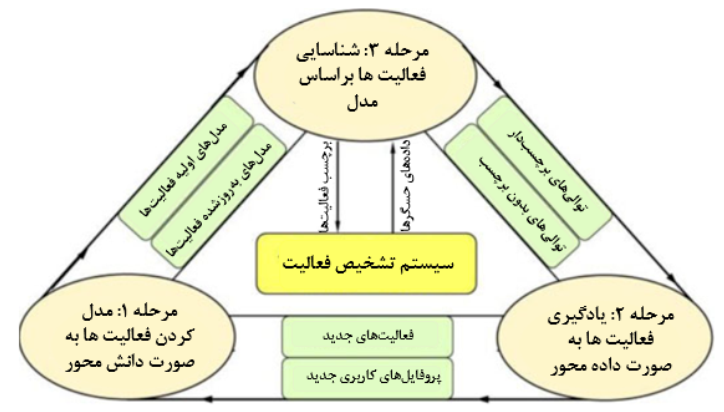
\includegraphics [width=\textwidth] {figs/f31.png}}
\caption[فرایند سه مرحله‌ای تکرارشونده‌ی مدل کردن فعالیت‌ها در راهکار چن و همکاران]{فرایند سه مرحله‌ای تکرارشونده‌ی مدل کردن فعالیت‌ها در راهکار چن و همکاران \cite{x3223}}
\label{fig:f31}
\end{figure}

\پاورق{‌عبدالصکور}{A. Sukor} و همکاران \cite{x3234} برای غلبه بر مشکل ناکامل بودن و به‌روز نبودن دانش فرد خبره، از ترکیب هستی‌شناسی و دسته‌بندهای بیز ساده، ماشین بردار پشتیبان و \پاورق{‌شبکه عصبی پرسپترون چند لایه}{Multi-layer perceptron neural network} استفاده کرده‌اند. از آنجایی که به دلیل خرابی حسگرها و یا تغییر شیوه انجام فعالیت‌ها توسط کاربران سیستم دچار خطا و عدم قطعیت می‌شود، رودریگز و همکاران \cite{x3228} یک \پاورق{‌منطق فازی}{Fuzzy logic} برای نمایش فعالیت‌ها ارائه کردند که امکان مدل‌سازی دانش غیرقطعی و مبهم را دارد. به این صورت که بر خلاف منطق دودویی که در آن هر عبارت به غلط یا درست قابل ارزیابی است، از \پاورق{‌منطق فازی}{Fuzzy logic} استفاده می‌کند که میزان درستی هر عبارت مقداری بین صفر تا یک است.

\پاورق{‌گایاتری}{Gayathri} و همکاران \cite{x3235} از ترکیب هستی‌شناسی و \پاورق{شبکه منطق مارکوف}{Markov logic network} استفاده کرده‌اند. به این صورت که تی‌باکس به \پاورق{‌منطق مرتبه اول}{First order logic} تبدیل می‎شود و با استفاده از نمونه‌های موجود در ای‌باکس، وزن‌ها محاسبه می‌شوند تا به فعالیت‌ها در شبکه منطق مارکوف، وزنی اختصاص یابد و توالی احتمالاتی فعالیت‌ها را داشته باشند.

راهکار دیگری توسط ریبونی و همکاران \cite{x3236} مطرح شد که با استفاده از استنتاج روی هستی‌شناسی، همبستگی معنایی بین فعالیت‌ها و نتایج رخداد هر یک استخراج می‌شود، سپس با استفاده از اطلاعات به دست آمده، فعالیت کاندید بعدی را شناسایی می‌کند.
برخی فعالیت‌ها الگوهای مشابهی دارند و سیستم‌های مطرح شده در تشخیص دقیق این فعالیت‌ها ممکن است با مشکل مواجه شوند. در راهکار دیگر که توسط \پاورق{‌بتینی}{Bettini} و همکاران \cite{x3237} مطرح شده است، شناسایی فعالیت‌ها به کمک حسگرهای تلفن همراه انجام می‌شود و برای این منظور از \پاورق{یادگیری نیمه‌نظارتی}{Semi-supervised learning} و استنتاج مبتنی بر هستی‌شناسی و همچنین اطلاعات زمینه‌ای استفاده نی‌شود. در این راهکار داده‌های دریافت شده از حسگرها که با اطلاعات زمینه‌ای نظیر مکان کاربر، طبق روابط معنایی تعریف شده در هستی‌شناسی همخوانی ندارند حذف شده و در گام آخر، اگر میزان اطمینان فعالیت شناسایی شده از حد مشخصی کمتر باشد، از کاربر استعلام فعالیت کنونی را گرفته و برچسب‌گذاری انجام می‌گردد. با انجام این فرایند، مدل همواره در حال یادگیری و به‌روز شدن است.

\subsection{جمع‌بندی}

در این بخش، پژوهش‌های انجام شده در حوزه مدل‌سازی و تشخیص فعالیت‌های کاربران در خانه‌های هوشمند بررسی و از نظر نوع رویکرد در دریافت اطلاعات مورد نیاز دسته‌بندی شدند. مقایسه‌ی کلی پژوهش‌های مطرح شده در جدول \ref{tab:t32} قابل مشاهده است.

\begin{table} [htp]
 \centering
 \caption{مقایسه‌ کلی روش‌های ترکیبی}
 \label{tab:t32}
 \begin{adjustbox}{width=\textwidth}
\begin{tabular}{|c|c|c|c|c|c|c|c|c|c|}
  \hline
  \multirow{3}{*}{\textbf{پژوهش}} & \multirow{3}{*}{\textbf{راهکار}} & \multicolumn{8}{c|}{\textbf{چالش‌ها}} \\
  \cline{3-10}
  & & \multicolumn{3}{>{\centering}m{0.18\textwidth}|}{\textbf{محدودیت‌های راهکارهای دانش‌محور}} & \multicolumn{3}{>{\centering}m{0.18\textwidth}|}{\textbf{محدودیت‌های راهکارهای داده‌محور}} & \multicolumn{2}{>{\centering}m{0.13\textwidth}|}{\textbf{پیچیدگی‌های شناسایی فعالیت}} \\
  \cline{3-10}
  & & \rotatebox[origin=c]{90}{\textbf{ناکامل بودن دانش فرد خبره}} & \rotatebox[origin=c]{90}{\textbf{عدم به روز شدن خودکار}} & \rotatebox[origin=c]{90}{\textbf{عدم توانایی در مواجهه با عدم قطعیت}} & \rotatebox[origin=c]{90}{\textbf{شروع سرد}} & \rotatebox[origin=c]{90}{\textbf{عدم امکان استفاده مجدد}} & \rotatebox[origin=c]{90}{\textbf{   ناکامل بودن مدل ایجاد شده توسط روش‌های یادگیری   }} & \rotatebox[origin=c]{90}{\textbf{امکان حضور چند کاربر}} & \rotatebox[origin=c]{90}{\textbf{شناسایی فعالیت‌های همزمان}} \\
  \hline
  \hline
چن و همکاران \cite{x3232,x3233} & یادگیری مبتنی بر داده‌کاوی &
\cmark & \cmark & \xmark & \cmark & \cmark & \cmark & \xmark & \xmark \\ 
  \hline
عبدالصکور و همکاران \cite{x3234} & ماشین بردار پشتیبان و شبکه عصبی پرسپترون &
\cmark & \cmark & \xmark & \cmark & \cmark & \cmark & \xmark & \xmark \\ 
  \hline
رودریگز و همکاران \cite{x3228} & منطق فازی &
\xmark & \xmark & \cmark & \cmark & \cmark & \cmark & \cmark & \cmark \\ 
  \hline
گایاتری و همکاران \cite{x3235} & شبکه منطق مارکوف &
\xmark & \xmark & \cmark & \cmark & \cmark & \cmark & \xmark & \cmark \\ 
  \hline
ریبونی و همکاران \cite{x3236} & روش‌های آماری و شبکه منطق مارکوف &
\xmark & \xmark & \xmark & \cmark & \cmark & \cmark & \xmark & \cmark \\ 
  \hline

\end{tabular}
\end{adjustbox}
\end{table}

\section{حفظ حریم خصوصی مبتنی بر سکوی نامعتمد}\label{chapter:c33}

تاکنون پژوهش‌های زیادی در جهت حفظ حریم خصوصی کاربر در حوزه‌‌‌های مختلف صورت پذیرفته است. مانند تحقیقاتی که در حوزه حفظ حریم خصوصی کاربر در \پاورق{‌داده کاوی}{Data mining}، انتشار اطلاعات، واکشی اطلاعات، و شبکه‌‌‌های نا‌‌‌امن صورت گرفته است. از منظر سکوهای اینترنت اشياء نیز حفظ حریم خصوصی کاربر در ابعاد مختلف بررسی شده است مانند امنيت در محل ذخیره سازی داده‌‌‌ها، امنيت در واکشی، اعتبارسنجی داده‌‌‌هایی که در سکو ذخیره می‌‌‌گردد و حفظ محرمانگی داده‌های کاربران در سرويس‌دهنده و يا سکوی نامعتمد \cite{x301}. این موضوع بیانگر جنبه‌‌‌های امنيتی گسترده‌ای است که کاربر را با تهدید مواجه می‌نماید. 

راهکارهایی که در هر یک از حوزه‌های مورد اشاره ارائه شده است بعضاً قابل تعمیم به حوزه‌‌‌های دیگر هم هستند. برای مثال در حوزه داده کاوی (که بر ذخیره داده‌‌‌های کاربران در طول زمان بر روی سکوهای ابری و انجام استنتاج‌‌‌های مربوطه و کلاسه‌بندی‌‌‌های مورد نیاز، اشاره دارد) یکی از تکنیک‌های حفظ امنیت کاربران، جلوگیری از استنتاج‌‌‌های غیر ضروری با استفاده از آشفته‌سازی داده‌‌‌های ذخیره شده در سکو است. همین راهبرد در برخی از راهکارهای حفظ حریم خصوصی کاربر در انتشار داده، به کار رفته است. ضمنا باید به این نکته نیز توجه داشت که پیاده‌‌‌سازی همه راهکارها، در اختیار کاربر نیست و در برخی راهکارها مستلزم همکاری سرویس‌دهنده، سکو و یا ارائه دهنده خدمات شبکه است. به طور مثال استفاده از رمزنگاری برای حفظ حریم خصوصی نیازمند همکاری بخش‌های مختلفی در زیرساخت اینترنت اشیاء است ولیکن روشی مانند آشفته‌سازی داده‌ها می‌تواند توسط عوامل تحت اختیار کاربر انجام پذیرد.

بسیاری از پژوهش‌های حفظ حریم خصوصی، با مدل تهدید سکوی نامعتمد انجام شده است که بر اساس راهکار، به دسته‌های مبتنی بر رمزنگاری، مبتنی بر کمینه‌سازی، مبتنی بر آشفته‌سازی داده و مبتنی بر تولید رویداد جعلی تقسیم می‌شوند. در این مدل تهدید فرض می‌شود که داده‌های حساس همواره در معرض خطر قرار دارند همانطور که تعداد بسیاری حمله با استفاده از این داده‌های حساس انجام شده است \cite{x3301,x3302}. به دلیل متمرکز بودن سکوها و دسترسی به تمامی داده‌های حساس توسط سکوها، مهاجمین توجه ویژه‌ای به آن‌ها می‌کنند. ضمن این که سکوها با داشتن دسترسی به تمامی اطلاعات خانه‌هوشمند و جمع‌آوری داده‌‌‌های محرمانه کاربر (که بعضا به آن نیاز ندارند)، می‌توانند از آن‌ها برای اهدافی مانند تبلیغات یا فروش به شرکت‌های دیگر استفاده کنند \cite{x3303,x3304}. راهکارهای ارائه شده در این حوزه را می‌توان به دسته‌های مختلفی تقسیم نمود که در ادامه به معرفی راهکارهای ارائه شده در هر دسته و تحلیل آن‌ها پرداخته شده است.

\subsection{راهکارهای مبتنی بر رمزنگاری}

یکی از روش‌های حفظ حریم خصوصی در برابر سکوی نامعتمد، استفاده از یک یا چند روش رمزنگاری روی داده‌هاست به نحوی که تمامی داده‌ها از دید سکو پنهان شود.

\پاورق{‌شوتلر}{Schoettler} و همکاران \cite{x3332} سکویی دو بخشی به نام \پاورق{‌والنات}{Walnut} تعریف کرده‌اند که هیچ کدام دسترسی به داده‌های حساس بخش دیگر ندارند. در این روش از تلفیق محاسبه دو جانبه امن و محیط اجرای امن به ترتیب برای حفظ محرمانگی و صحت استفاده می‌شود. این پژوهش فقط مدل ارتباطی رویداد-کنش را در نظر گرفته است و مدل ارتباطی رویداد-محاسبه-کنش را در نظر نمی‌گیرد.

در پژوهش دیگری، \پاورق{‌زاوالیشن}{Zavalyshyn} و همکاران \cite{x3331} از طریق معرفی یک سکوی معتمد با معماری جدید به نام \پاورق{‌پاترآی‌اتی}{PatrIoT}، سعی بر حفظ حریم خصوصی کاربر را دارند. این پژوهش مانند والنات از محیط اجرای امن استفاده کرده است. همچنین این پژوهش یک لایه محافظتی مبتنی بر خط مشی ارائه کرده است که کنترل جریان‌های داده از دستگاه‌ها تا سکو و حذف جریان‌های نامطلوب از دید کاربر را بر عهده دارد.

در پژوهش دیگری، \پاورق{‌چیانگ}{Chiang} و همکاران \cite{x3321} معتقدند که سکو به کمک داده‌های دریافتی، برای هر کاربر پروفایل اختصاصی درست می‌کند. داده‌های ارسال شده توسط هر نرم‌افزار، استفاده یا عدم استفاده از دستگاهی خاص مانند دستگاه اندازه‌گیری قند خون و حتی عدم دریافت داده مورد انتظار از یک برنامه در زمان مشخص، اطلاعات حساسی هستند که سکو به آن‌ها دسترسی دارد. برای مبهم‌سازی اطلاعات در این پژوهش دو راهکار \پاورق{‌\lr{OTAP}}{Obfuscated Trigger-Action Platform} و \پاورق{‌\lr{ATAP}‌}{Anonymous Trigger-Action Platform} ارائه شده است. \lr{OTAP} اطلاعات وقوع یا عدم وقوع رخدادها را از سکو پنهان می‌کند. با استفاده از رمزنگاری \پاورق{‌انتها به انتها‌}{End-to-End} بین رویداد و کنش، اطلاعات را از سکو پنهان می‌کند. \lr{ATAP} علاوه بر انجام راهکارهایی که \lr{OTAP} ارائه می‌دهد، اطلاعات مالکیت را نیز پنهان می‌کند. با استفاده رمزنگاری متقارن بین سرویس رویداد و کنش، سعی در مخفی نگه داشتن پروفایل کاربران دارد و داده‌ای که در اختیار سکو قرار می‌گیرد تنها به سرویس کنش تحویل داده می‌شود. این پژوهش نیز مانند پژوهش \پاورق{‌ژو}{Xu} و همکاران \cite{x3311}، دستگاه‌هایی که مستقیما و بدون واسط با سکو در ارتباط هستند را در نظر نگرفته است. در این پژوهش تنها الگوی رویداد-کنش در نظر گرفته شده است در صورتی که ممکن است الگوی رویداد-محاسبه-کنش مورد استفاده‌ باشد.

در پژوهش دیگری، چن و همکاران \cite{x3322} \پاورق{‌\lr{eTAP}}{Encrypted Trigger Action Platform} را معرفی کرده‌اند. سکوی معرفی شده محاسبات مورد نیاز را روی داده‌های رمز شده انجام داده و قابلیت استنتاج از نتیجه‌ی محاسبات را ندارد. در مدل تهدید این پژوهش مهاجم ممکن است فعال باشد. ضعف این پژوهش عدم پنهان‌سازی وقوع یا عدم وقوع رخدادهاست که علی‌رغم رمزنگاری، توسط مهاجم قابل تشخیص است.

\subsection{راهکارهای مبتنی بر کمینه‌سازی}

در روش‌های ارائه شده مبتنی بر کمینه‌سازی، به طور کلی در خروجی سيگنال‌های سری زمانی حسگرهای يک خانه هوشمند، بخش مربوط به فعاليت‌های حساس کاربر حذف می‌‌‌گردد و به جای آشفته سازی، خروجی برش می‌‌‌خورد. برای مثال در یکی از راهکارهایی که در این دسته قرار می‌‌‌گیرد انتشار جریان زمینه کاربر برای حفظ حریم خصوصی وی به انتخاب کاربر منقطع می‌‌‌گردد و در هر زمینه جدید، در مورد انتشار و یا عدم انتشار اطلاعات تصمیم گیری می‌‌‌شود \cite{x3121}. به عنوان مثالی در اين حوزه، فرض کنید که کاربر مایل باشد که از سرویس ساکت شدن زنگ موبایل خود هنگامی که در جلسه کاری است استفاده کند اما در لحظات دیگر تمایلی نداشته باشد که سرویس دهنده از شرایط محلی که وی در آن حضور دارد مطلع شود و مثلاً متوجه نشود که کاربر در خانه است، در حال رانندگی کردن است و یا در حال قدم زدن است. 

روش کمینه‌سازی شناسایی فعاليت‌های حساس کاربر را برای مهاجم دشوار می‌‌‌نمايد اما همچنان فاصله‌‌‌های زمانی انجام فعاليت‌های حساس کاربر و در مواردی حتی شناسایی خود فعاليت‌ها را برای مهاجم ميسر می‌نماید. مثال‌های گوناگونی در این حوزه وجود دارند که چگونگی نشت اطلاعات محرمانه از روی داده‌‌‌های غیر محرمانه را به کمک روش‌های مهندسی اجتماعی و یا مدل‌سازی رفتار کاربر در طول زمان توسط مهاجم (به کمک مدل زنجیره مارکوف) را نشان می‌‌‌دهند \cite{x3121}. در ضمن با حذف بخشی از سری زمانی مربوط به سيگنال‌ها، بخشی از اطلاعات مربوط به فعاليت‌های غيرحساس کاربر نیز ممکن است حذف شود و به اين ترتیب از کارايي داده‌‌‌های ارسالی به سکوهای اينترنت اشياء کاسته می‌‌‌شود. همچنین تکنیک‌های کمینه‌سازی که بخواهند تحلیل کاملی را روی داده قبل از ارسال آن انجام دهند ممکن است با مشکلات پردازشی و تجربه بد کاربری روبرو شوند. مشکل دیگر روش‌های کمینه‌سازی این است که برای دریافت برخی سرویس‌ها (مثلا اتوماسیون امور با استفاده از برنامه‌های اینترنت اشیاء) لازم است که داده‌هایی به سکو الزاما ارسال شود که از دید کاربر بخشی از آن‌ها حساس و محرمانه است. لذا یک تعارض بین دریافت سرویس از سکوی اینترنت اشیاء و حفظ حریم خصوصی پیش می‌آید که این دسته از روش‌ها قادر به رفع این تعارض نیستند و باید از روش‌های دیگری برای حفظ حریم خصوصی استفاده کرد.

ژو و همکاران \cite{x3311} ارتباط بین سکوی اسمارت‌تینگز و سکوهای شخص ثالث مانند ایفت را بررسی کرده‌اند و به این نتیجه رسیده‌اند که سکوی شخص ثالث به اطلاعات زیادی دسترسی دارد که به نوعی نقض حریم خصوصی کاربر محسوب می‌شود. در این پژوهش با استفاده از ماژولی به نام \پاورق{‌\lr{F\&F}}{Filter \& Fuzz} برای مبهم‌سازی الگوی اطلاعات دریافتی، اطلاعات جعلی ایجاد می‌شود. همچنین در مواردی که سکو برای کنش، نیاز به اطلاعات دقیق ندارد، داده‌های تقریبی و دستکاری شده برای سکو ارسال می‌گردد. مهمترین چالش این پژوهش این است که سکوی اسمارت‌تینگز مورد اعتماد فرض شده و فقط سکوی ثالث نامعتمد است.

در پژوهشی دیگر، \پاورق{‌چی}{Chi} و همکاران \cite{x3312} سیستم کنترل جریان داده‌ای به نام \پاورق{‌پی‌فایروال}{PFirewall} معرفی کرده‌اند. این ابزار ابتدا کد برنامه‌ی اینترنت اشیاء در هر دستگاه را بررسی کرده و سپس داده‌ی مورد نیاز برای ارسال رویدادهای هر یک را استخراج می‌کند. با این کار تنها داده‌های مورد نیاز به سکو ارسال شده و از ارسال داده‌های اضافی جلوگیری می‌شود. مزیت این ابزار آن است که نیازی به تغییر سکو، هاب و یا دستگاه‌ها نیست و ابزار پی-فایروال بین هاب و سکو قرار می‌گیرد. همانطور که در بخش \ref{chapter:c24} گفته شد برخی دستگاه‌ها مستقیما با سکو در ارتباط هستند و این پژوهش این دسته از دستگاه‌ها را در نظر نگرفته است. همچنین ممکن است کد برنامه‌ی اینترنت اشیاء در تمامی دستگاه‌ها در دسترس نباشد و پی‌فایروال قادر به استخراج اطلاعات مورد نیاز نباشد.

در پژوهشی دیگر، چن و همکاران \cite{x3121Z} با ارائه \پاورق{‌‌مین‌تپ}{minTAP} کارایی روش کمینه‌سازی را افزایش دادند. در این پژوهش کاربر قواعد را تعریف کرده و سپس با پردازش روی این قواعد، اطلاعات کمینه‌سازی استخراج شده و به همراه قواعد به سکو ارسال می‌شود. هنگام رخداد رویداد، خصیصه‌های آن به همراه کمینه‌ساز به سرویس‌دهنده ارسال شده و اطلاعات اضافه از رویداد حذف شده و سپس به سکو ارسال می‌گردد. این راهکار کارایی بالا و سربار قابل قبولی دارد اما نیاز به اعمال تغییرات سمت سرویس‌دهنده است.

راهکار دیگری که مبتنی بر کمینه‌سازی ارائه شده است، استفاده از \پاورق{‌نگاشت}{Mapping} است که در این روش‌ها به کمک اعمال محدوديت‌ها بر روی سری‌‌‌های زمانی، سری‌‌‌های زمانی جديدی از خروجی حسگرها ايجاد می‌‌‌گردد \cite{x3131}. و غالباً اطلاعات سری زمانی اوليه حسگرها به فضای حالتی با ابعاد کوچکتر نگاشت می‌گردد تا از ميزان اطلاعاتی که به همراه دارد کاسته شود. در اين روش به جای ارسال سری زمانی با ابعاد بالا (مثلا یک حسگر مربوط به سیستم تهویه مطبوع ممکن است ويژگی‌‌‌هایی مانند وضعیت عملکرد فعلی، شدت فن، و دمای محیط را ارسال نماید)، فقط بخشی از ویژگی‌های اصلی از خروجی حسگرها استخراج شده و ارسال می‌‌‌شود به نحوی که داده‌‌‌ها فقط برای استنتاج فعاليت‌های غيرحساس مفيد واقع شود. در یکی از راهکارهایی که در این دسته پیشنهاد شده است، داده‌‌‌های کاربر قبل از ارسال، پیش پردازش می‌‌‌گردد تا فقط داده‌‌‌هایی که برای دريافت سرویس‌‌‌های داده کاوی خاص از سکو مورد نیاز است، ارسال شود. بدین ترتیب برای مثال اگر تجهیزی برای شناسایی حرکت در خانه استفاده می‌‌‌گردد، برای استنتاج این موضوع که آیا شخصی در خانه حضور دارد یا خیر نمی‌تواند مورداستفاده قرار گیرد. در این راهکار از يک ماژول استخراج کننده ويژگی به کمک شبکه عصبی استفاده شده است تا با کمک تکنیک‌های کاهش ابعاد، ساختار داده اصلی حفظ شود و فقط آنچه لازم نیست حذف گردد و این امر با کم کردن فاصله معنایی ويژگی‌‌‌های مربوط به هم و افزایش فاصله معنایی ويژگی‌‌‌های غیرمرتبط با هم صورت می‌‌‌گیرد. مثلا جنسیت کاربر توسط سکو شناسایی می‌‌‌شود اما تصویر وی شناسایی نمی‌‌‌گردد \cite{x3131}. 

قسمت دشوار استفاده از راهکار نگاشت، انتخاب بهترين مجموعه کوچک ويژگی به خصوص در روش‌های متکی بر يادگيری ماشين است که بتواند يک توازن منطقی بين کارایی داده‌‌‌های ارسالی و حفظ حریم خصوصی ايجاد نمايد. در راهکار ديگری که در اين دسته ارائه شده است داده‌‌‌های مربوط به سری زمانی در هر مقطع از زمان طی یک فرآیند آماری به صورت تصادفی نگاشت می‌‌‌گردد و اين نگاشت به نحوی صورت می‌‌‌گیرد که کاربردپذيری خروجی را به صورت حداکثری نگاه دارد. هدف از انجام اين نگاشت اين است که نمونه‌‌‌های داده سری‌‌‌ زمانی در طول زمان مستقل از هم بشوند و همبستگی خود را از ديد مهاجم بیرونی مخفی نمايند \cite{x3132}. چالشی که در این دسته از راهکارها وجود دارد این است که ممکن است برخی از سرويس‌های سکوها، با سيگنال‌هایی که ويژگی‌‌‌های اصلی آن‌ها تغییر يافته است نتوانند کار کنند. در ضمن در اين روش اصلا نمی‌‌‌توان تضمين نمود که هر ويژگی در مجموعه‌‌‌ای که انتخاب شده است تنها حاوی اطلاعات يک فعاليت غیرحساس باشد و هيچ اطلاعی از يک فعاليت حساس را به همراه نداشته باشد. 

\subsection{راهکارهای مبتنی بر آشفته‌سازی}

در اين روش هدف ارسال داده تفییریافته است به شکلی که کاربر بتواند سرویس‌های دلخواه خود را از سکو یا سرویس دهنده دریافت نماید و در عین حال عدم قطعیت داده تضمین گردد \cite{x3111}. منظور از عدم قطعیت داده اين است که از روی داده‌‌‌های آشفته، ساخت اصل داده‌‌‌ها میسر نباشد. 

تنوع راه‌‌‌حل‌‌‌ها و چالش‌ها در این دسته از راهکارها زیاد است و بررسی‌‌‌های متعددی در اين خصوص صورت گرفته است برای مثال مطالعاتی در خصوص اعمال انواع مختلف نويز به داده‌‌‌های سری زمانی حسگرها، مانند اعمال نویز تصادفی با الگوریتم‌های مختلف \cite{x3113,x3112}، اعمال نویزی که با سری زمانی اصلی همبستگی دارد \cite{x3114}، اعمال نویز در کنار فشرده‌‌‌سازی سیگنال اولیه \cite{x3113}، و یا اعمال نویز با توجه به حفظ فاصله اقلیدسی‌‌‌ سیگنال‌های حسگرهای مشابه از کاربران مختلف \cite{x3112} صورت گرفته است و مزایا و معایب هر روش پیشنهادی با توجه به معیارهایی که برای اندازه‌‌‌گیری حفظ حریم خصوصی کاربر و کاربردپذیری سیگنال تعریف شده اندازه‌‌‌گیری شده است. 

در کنار این راهکارها، روش‌هاي متعددی نيز برای بازسازی داده‌‌‌های اولیه از روی داده‌‌‌های آشفته‌سازی‌شده پيشنهاد شده است که نقاط ضعف استفاده از این راهکارها را به چالش کشیده است \cite{x3112,x3115,x3116}. به طور خلاصه در مورد این راه‌‌‌حل‌ها می‌‌‌بایست گفت که میزان نویز اعمال شده به سیگنال اولیه، قابلیت کاربرد پذیری سیگنال (منظور امکان استفاده کاربر از سرویس‌های دلخواه) را به شدت تحت تاثیر قرار می‌‌‌دهد و حتی ممکن است اصل داده‌‌‌ها را تخریب نماید. بسیاری از راهکارهای این دسته شناسایی فعاليت‌های حساس کاربر را برای مهاجم با دشواری مواجه می‌‌‌کنند اما عدم قطعیت داده را تضمین نمی‌‌‌کنند.

راهکار دیگری برای آشفته‌سازی داده، استفاده از \پاورق{‌جایگزینی}{Replacement} است. در این روش، بخش حساس سری‌‌‌های زمانی با داده‌‌‌های غيرحساس جايگزين می‌‌‌گردد. برای مثال در یکی از رويکردهايي که در این دسته ارائه شده است \cite{x3141} به کمک تکنيک‌‌‌های يادگيری ماشين، رفتارهای حساس کاربر با رفتارهای غيرحساس جايگزين می‌‌‌گردد. در اين راهکار فعاليت‌های کاربر به دو گروه سفيد (غیر حساس) و سياه (حساس) تقسیم می‌‌‌گردد. منظور از رفتارهای حساس کاربر رفتارهايي هستند که برخی از حالات روانشناسی کاربر مانند وجود استرس از آن‌ها قابل استخراج است. شبکه پویای بیزین پیشنهادی در این روش، آموزش می‌‌‌بیند و در مرحله اول برای شناسايي بلاک‌های حساس کاربر در سیگنال‌های خروجی استفاده می‌‌‌گردد. سپس در مرحله بعد برای انتخاب بخش‌هایی که می‌‌‌بایست جایگزین بلاک‌های حساس گردد، استفاده می‌‌‌گردد. البته با حفظ این محدودیت که طول بلاک‌هایی که حذف می‌‌‌گردد با طول بلاک‌هایی که جایگزین می‌‌‌گردد مساوی باشد. در این راهکار توسط ماژولی سیگنال خام ورودی به سیگنالی مبتنی بر ويژگی‌‌‌های رفتاری تبديل می‌‌‌شود و با حذف رفتارهای حساس تعدادی حفره باقی می‌‌‌مانند که می‌‌‌بایست توسط رفتارهای غیرحساس پر شوند و جایگزینی به نحوی صورت می‌‌‌گیرد که به تداوم جریان سیگنال لطمه وارد نشود. برای جایگزینی رفتارها از یک پایگاه داده نگاشت رفتاری با طول‌های زمانی مختلف استفاده می‌‌‌گردد. اين راهکار به صورت برون-خط عمل می‌‌‌کند یعنی قبل از تصميم‌‌‌گيری برای جايگزينی، اطلاعات سری‌‌‌زمانی فعاليت کاربر می‌‌‌بایست در دسترس باشد. 

به عنوان مثالی ديگر از راهکارهای این دسته به راهکار ارائه شده در پژوهش آقای ملک زاده \cite{x3142} می‌‌‌توان اشاره کرد که در آن يک شبکه عصبی آموزش ديده به نام \پاورق{‌خودرمزگذار}{َAutoEncoder} جایگزین‌کننده، عملی مانند رفع نويز انجام می‌‌‌دهد و الگوریتم جایگزینی فعاليت‌های حساس با فعاليت‌های غيرحساس را انجام می‌‌‌دهد به نحوی که امکان تشخیص و استنتاج فعاليت‌های حساس از بین می‌‌‌رود. داده‌ها در این راهکار به سه دسته‌ی سیاه (حساس)، خاکستری (غیر حساس است و استنتاج این رفتار برای کاربر مهم نیست) و سفید (غیر حساس است و استنتاج این رفتار برای کاربر مهم و کاربردپذیر است) تقسیم می‌شوند. در هر سری زمانی و بازه‌ی دلخواه، الگوریتم مطرح شده با در نظر گرفتن کاربردپذیری از بعد دريافت سرويس‌های مد نظر کاربر از سکو، داده‌هایی از لیست سیاه را با خاکستری جایگزین می‌کند. در این راهکار اثبات می‌‌‌شود که مهاجم بدون داشتن داده‌های مورد استفاده برای تعلیم لیست خاکستری، امکان تشخیص داده‌های حساس را ندارد و از کاربردپذیری داده‌‌‌های ارسالی به سکوهای اينترنت اشياء برای دريافت سرويس‌های دلخواه کاسته نمی‌‌‌شود.

\subsection{راهکارهای مبتنی بر تولید رویدادهای جعلی‌}‌

در پژوهش‌های مبتنی بر تولید رویداد جعلی، برای حفظ حریم خصوصی کاربر، به جای حذف، تغییر یا پنهان‌سازی داده، از اضافه کردن داده‌های جعلی برای گمراه کردن سکو استفاده می‌شود. تولید و ارسال داده‌های جعلی در این پژوهش‌ها به نحوی است که سکو امکان تمایز این داده‌ها با داده‌های واقعی را نداشته باشد و از طرفی کنش‌های سکو در جواب رویدادهای جعلی اعمال نشود.

در پژوهش ژو و همکاران \cite{x3311} الگوهای آماری باعث نقض حریم خصوصی می‌شود و برای عدم استنتاج سکو، تعدادی رویداد جعلی با برچسب مشخص ارسال می‌شود و از آن‌جایی که سکو قادر به تمایز میان رویدادهای جعلی و حقیقی نیست، کنش‌های مرتبط را ایجاد می‌کند. در آخر، با توجه به برچسب هر رویداد و وابستگی کنش‌ها به رویدادها، کنش‌های ناشی از رویدادهای جعلی تشخیص داده شده و کنار گذاشته می‌شوند.

در پژوهش چیانگ و همکاران \cite{x3321}، محرمانگی داده‌های ارسالی به سکو تضمین شده است اما در بسیاری از موارد، وقوع یا عدم وقوع یک رویداد، یک داده‌ی حساس به شمار می‌آید. برای پنهان کردن این اطلاعات، از رویکرد تولید رویداد جعلی استفاده شده است که به صورت متناوب، در بازه‌های زمانی مشخص، هر دستگاه اینترنت اشیاء، داده‌های جعلی و حقیقی را با هم به سکو ارسال می‌کند.

اقوامی‌پناه و امینی\footnote{آزمایشگاه امنیت داده و شبکه، دانشگاه صنعتی شریف} \cite{x3341} برای فریب مهاجمی که با استفاده از شبکه عصبی \پاورق{‌\lr{LSTM}}{Long-Short Term Memory} اقدام به استنتاج فعالیت‌های کاربر می‌کند، راهکاری بر اساس تولید رویدادهای جعلی ارائه کرده‌اند\footnote{مقاله پژوهش تا زمان نگارش این مطلب منتشر نشده است.}. در این پژوهش با استفاده از \پاورق{نمونه ‌خصمانه}{Adversarial example} و تولید رویدادهای جعلی در بازه‌های زمانی مشخص، جلوی استنتاج مهاجم گرفته می‌شود. همچنین، کنش‌هایی که در نتیجه‌ی رویدادهای جعلی دریافت می‌شود کنار گذاشته می‌شود تا کاربردپذیری خانه هوشمند کاهش پیدا نکند. هرچند این پژوهش در ابتدا فرض را بر استفاده‌ی سکو از شبکه عصبی \lr{LSTM} برای استنتاج فعالیت‌های کاربر قرار داده است؛ ولیکن در ادامه با بررسی قابلیت انتقال‌پذیری، امکان موثر بودن نمونه‌های خصمانه تولید شده در به اشتباه انداختن دسته‌بندهای مبتنی بر روش‌های دیگر را با انجام آزمایش‌های عملی به اثبات رسانده است. یکی از ضعف‌های این پژوهش این است که در صورت هوشمندی بیشتر سکوی مهاجم و تجهیز آن به برخی روش‌های شناسایی ناهنجاری، امکان تشخیص و شناسایی رویدادهای جعلی تولید شده با این روش و حذف آن‌ها وجود خواهد داشت. ضعف دیگر، وجود روش‌های دفاعی \cite{x3342} در مقابل نمونه‌های خصمانه است که موجب ناکارآمد شدن این راهکار در برابر مهاجم هوشمند می‌شود.

\subsection{جمع‌بندی}‌

در این بخش پژوهش‌های حفظ حریم خصوصی مبتنی بر سکوی نامعتمد بررسی شد که اکثرا نیاز به تغییر سکو و دستگاه‌ها دارند که سبب مشکل در استفاده شده است. در جدول \ref{tab:t33} می‌توان مقایسه کلی این روش‌ها را مشاهده کرد.

\begin{sidewaystable} [htp]
 \centering
 \caption{مقایسه‌ کلی روش‌های حفظ حریم خصوصی مبتنی بر سکوی نامعتمد}
 \label{tab:t33}
 \begin{adjustbox}{width=\textwidth}
 \begin{tabular}{|c|c|c|c|c|c|c|c|}
 \hline
 \textbf{پژوهش} & \textbf{راهکار} & \textbf{پشتیبانی از محاسبه} & \textbf{عدم تغییر سرویس‌ها} & \textbf{عدم تغییر سکو} & \textbf{سربار قابل قبول} & \textbf{حفظ کاربردپذیری} & \textbf{حفاظت در برابر مهاجم هوشمند} \\
 \hline \hline
ژو و همکاران (\lr{F\&F}) \cite{x3311} & کمینه‌سازی، آشفته‌سازی و تولید رویدادهای جعلی & 
\cmark & \cmark & \xmark & \cmark & \cmark & \xmark \\
 \hline
چی و همکاران (\lr{PFirewall}) \cite{x3312} & کمینه‌سازی & 
\cmark & \cmark & \cmark & \cmark & \xmark & \xmark \\
\hline
چیانگ و همکاران (\lr{OTAP}) \cite{x3321} & رمزنگاری و تولید رویدادهای جعلی & 
\xmark & \xmark & \cmark & \xmark & \cmark & \cmark \\
\hline
چیانگ و همکاران (\lr{ATAP}) \cite{x3321} & رمزنگاری و تولید رویدادهای جعلی & 
\xmark & \xmark & \xmark & \cmark & \cmark & \cmark \\
\hline
چن و همکاران (\lr{ETAP}) \cite{x3322} & رمزنگاری & 
\cmark & \xmark & \xmark & \xmark & \cmark & \cmark \\
\hline
چن و همکاران (\lr{minTAP}) \cite{x3121Z} & کمینه‌سازی & 
\cmark & \xmark & \cmark & \cmark & \xmark & \xmark \\
\hline
زاوالیشن و همکاران (\lr{PatrIoT}) \cite{x3331} & رمزنگاری & 
\cmark & \cmark & \xmark & \xmark & \cmark & \cmark \\
\hline
شوتلر و همکاران (\lr{Walnut}) \cite{x3332} & رمزنگاری & 
\cmark & \xmark & \xmark & \xmark & \cmark & \cmark \\
\hline
ملک‌زاده و همکاران \cite{x3142} & آشفته‌سازی & 
\cmark & \cmark & \cmark & \xmark & \xmark & \xmark \\
\hline
اقوامی‌پناه و امینی \cite{x3341} & تولید رویدادهای جعلی & 
\cmark & \cmark & \cmark & \xmark& \cmark & \xmark \\
\hline
\end{tabular}
\end{adjustbox}
\end{sidewaystable}








